\documentclass[11pt]{article}
\usepackage[T1]{fontenc}
\usepackage{lmodern,microtype,amsmath,amssymb,amsthm,mathtools,booktabs,array,xurl}
\usepackage[a4paper,margin=28mm]{geometry}
\usepackage{tikz}
\usetikzlibrary{arrows.meta,calc,positioning}
\usepackage[colorlinks=true,linkcolor=blue!55!black,citecolor=blue!55!black,urlcolor=blue!55!black]{hyperref}
\numberwithin{equation}{section}
\setlength{\emergencystretch}{2em}
\newtheorem{theorem}{Theorem}[section]
\newtheorem{proposition}[theorem]{Proposition}
\newtheorem{lemma}[theorem]{Lemma}
\newtheorem{corollary}[theorem]{Corollary}
\theoremstyle{definition}\newtheorem{definition}[theorem]{Definition}
\theoremstyle{remark}\newtheorem{remark}[theorem]{Remark}
\newcommand{\ii}{\mathrm i}
\newcommand{\dd}{\mathrm d}
\newcommand{\Vol}{\operatorname{Vol}}
\newcommand{\Rea}{\operatorname{Re}}
\newcommand{\Ima}{\operatorname{Im}}
\newcommand{\Turn}{\mathsf T}
\newcommand{\eps}{\varepsilon}
\newcommand{\CC}{\mathbb C}
\newcommand{\RR}{\mathbb R}
\newcommand{\diag}{\operatorname{diag}}
\newcommand{\Log}{\operatorname{Log}}
\newcommand{\kap}{\varkappa}
\title{Marked deformations and long fillings\\of Conway closures}
\author{}\date{}
\begin{document}\maketitle

\begin{abstract}
We deform the complete pyramid-and-prism construction of a
completed-root Conway closure. A holomorphic potential defined
directly from the cells gives the actual meridian and disk-longitude
logarithms on every crossing circle. Entire complex face maps retain
the original closed cut, all group relations and every parabolic
main cusp. The primitive equations have a unique small solution
for independently sufficiently long signed fillings. We verify
that the logarithmic meridian winds once, so the completion is the
original smooth filled exterior. The absolute volume is the real
part of a corrected critical action, with its constant fixed by
the original complete cell volumes. The proof is classical and
does not use a quantum packet or a noncancellation theorem.
\end{abstract}

\section{The marked exteriors and the filling theorem}
\label{cf:intro}

The starting link is specified by a finite ordered construction.
A two-string box has endpoints $0,1,2,3$ in cyclic order, starting
at the bottom left. In a vertical stack $FG$, the lower box $F$
is joined to the upper box $G$ by $F_2/G_1$ and $F_3/G_0$.
The exposed tuple is $(F_0,F_1,G_2,G_3)$.
A clockwise turn rotates the entire box and all its crossing disks;
the new tuple is $(F_1,F_2,F_3,F_0)$.
Cylindrical closure joins $0$ to $3$ and $1$ to $2$.

Let $h$ be the quarter-turn of an elementary crossing circle
surrounding two untwisted strands. The completed grammar is
\begin{equation}\label{cf:grammar}
 E::=hh\mid\Turn(E)\mid E_1E_2\mid hE\mid Eh,
 \qquad \text{closure }C(FG),\quad F,G\text{ completed}.
\end{equation}
Every leaf is a distinct crossing circle. Both closing children
must be completed; a bare closing leaf is not included.
Fix a retained half twist $\eps_\ell\in\{-1,0,1\}$ at each leaf.
The original augmented exterior is denoted $Y^\eps_E$.
Its crossing-circle meridian $\mu_\ell$ and disk longitude
$\lambda_\ell$ are fixed before any deformation.
They are the primitive curves of \cite[Section~7]{Geometry}.

For integers $p_\ell$, fill the auxiliary tori along
\begin{equation}\label{cf:slope}
       \mu_\ell+p_\ell\lambda_\ell .
\end{equation}
The physical crossing power in the original disk frame is
$n_\ell=\eps_\ell-2p_\ell$.
Indeed, cut along the twice-punctured disk and rotate one side
through $p_\ell$ full turns before removing its auxiliary circle.
The slope \eqref{cf:slope} becomes the meridian of the inserted
solid torus, and the strands acquire $-2p_\ell$ crossings.
These operations take place in the disjoint original leaf balls.
They preserve the ambient $S^3$ and give precisely the diagram
with these crossing powers. Write $Y^\eps_E(\mathbf p)$ for
its exterior. If the main endpoint matching is one component,
it is $S^3\setminus K_{\eps,\mathbf p}$.
Such half-twist choices exist by \cite[Proposition~8.1]{Geometry};
full twists preserve that component count.

We use two precise complete inputs. The strict stationary point
and its negative definite internal-wire Hessian are
\cite[Proposition~5.3]{Newton}, for the grammar \eqref{cf:grammar}.
The actual complete metric, its absolute volume $2\pi F_0$,
the labeled original cut and the primitive cusp basis are
\cite[Theorem~1.2 and Section~7]{Geometry}. At leaf $\ell$ its
complete angle $a_\ell$ satisfies
\begin{equation}\label{cf:cusp}
 \frac14<a_\ell<\frac{\arctan2}{\pi},\qquad
 \tau_\ell=\frac{2\ii c_\ell}{1-\eps_\ell\ii c_\ell},
 \quad c_\ell=\cot(\pi a_\ell),\quad \Ima\tau_\ell>0.
\end{equation}
Here $\tau_\ell$ is the longitude translation divided by the
meridian translation, with the orientation of the original torus.
No filled metric is an input.

Section~\ref{cf:potential} defines a holomorphic classical
potential $\Phi_\eps(\boldsymbol\chi)$ from these cells, with
$\Phi_\eps(0)=F_0$. Its variables are centered auxiliary
meridian coordinates, not the meridian of the main knot.

\begin{theorem}\label{cf:main}
For the fixed construction \eqref{cf:grammar} and fixed
half-twist pattern, there is a holomorphic framed representation
$\rho_{\boldsymbol\chi}$ of the original group
$\pi_1(Y^\eps_E)$ near $\boldsymbol\chi=0$. It continues the
oriented complete holonomy and has primitive similarity
logarithms
\begin{equation}\label{cf:UV}
 U_\ell=-2\pi\ii\chi_\ell,\qquad
 V_\ell=-2\,\partial_{\chi_\ell}\Phi_\eps .
\end{equation}
Every main peripheral group remains parabolic.
There is $B_E>0$ such that for every signed integer tuple with
$|p_\ell|>B_E$ the function
\begin{equation}\label{cf:action}
 S_{\eps,\mathbf p}(\boldsymbol\chi)
 =\Phi_\eps(\boldsymbol\chi)
       +\frac{\pi\ii}{2}\sum_\ell\frac{(\chi_\ell-1)^2}{p_\ell}
\end{equation}
has a unique critical point in a fixed small neighborhood of zero.
Its representation completes to a smooth oriented complete
finite-volume hyperbolic metric on the original
$Y^\eps_E(\mathbf p)$, and
\begin{equation}\label{cf:volume}
 \Vol\bigl(Y^\eps_E(\mathbf p)\bigr)
       =2\pi\Rea S_{\eps,\mathbf p}(\boldsymbol\chi_*).
\end{equation}
The bounds are independent of relative signs and relative sizes
of the $p_\ell$. Every main cusp is left complete.
\end{theorem}

Uniqueness here is local uniqueness in this prescribed family
and coordinate neighborhood. It does not classify the whole
character variety or all possible representations of the filled
group. The action in the theorem is defined geometrically below.
Identifying it with a particular finite quantum source is a
separate interface, described in Section~\ref{cf:interface}.

We import the general near-complete metric implication of
\cite[Proposition~6.1]{Marked}, after verifying every hypothesis
on this original family. We also use its local peripheral-volume
differential \cite[equation~(7.3)]{Marked} and the same-chain
comparison of \cite[Section~7.3]{Marked}. Neither import assumes
a source asymptotic. The normalizations and applicability are
made explicit in Sections~\ref{cf:metric}--\ref{cf:volume-proof}.

\section{A classical holomorphic cell potential}
\label{cf:potential}

\subsection{Logarithms, hidden leaf parameters and the half twist}
On a complex neighborhood of each strict real angle interval
continue the branch
\[
 J(u)=\int_0^u\Log(2\sin\pi s)\,\dd s
\]
from the real log-sine primitive. All occurrences are continued
from the fixed complete point, so their constants are fixed.
The product function is
\begin{equation}\label{cf:m}
\begin{split}
 m(x,y,z)={}&J(x+y)+J(z)-J(x)-J(y)\\
            &-J(z-x)-J(z-y)-J(x+y-z).
\end{split}
\end{equation}
Its strict complete domain is
$\max(x,y)<z<x+y<1$, with $x,y>0$.
For a leaf define
\begin{equation}\label{cf:g}
 g(x,t)=J(2x)-2J(x)-J(x-t)-J(x+t),\qquad
 v=g_t=\Log\frac{\sin\pi(x-t)}{\sin\pi(x+t)}.
\end{equation}
The parameter $t$ will be an auxiliary coordinate before the
half-twist shear. At $t=0$ this is the complete leaf action,
and $v=0$.

For $\eps=0,1,-1$ define $t=t(x,\chi)$ by
\begin{equation}\label{cf:shear}
 \chi=t-\frac{\eps v(x,t)}{2\pi\ii}.
\end{equation}
At $(x,t)=(a,0)$ its $t$ derivative is
$1-\eps\ii\cot\pi a\ne0$. The holomorphic implicit-function
theorem gives a unique small $t(x,\chi)$, with $t(x,0)=0$.
Set
\begin{equation}\label{cf:local-potential}
 f_\eps(x,\chi)
       =g(x,t)-\frac{\eps v(x,t)^2}{4\pi\ii}.
\end{equation}
The elementary differential calculation
\begin{equation}\label{cf:local-differential}
 \dd f_\eps=g_x\,\dd x+v\,\dd\chi
\end{equation}
is exact. The term subtracted in \eqref{cf:local-potential}
keeps the same boundary covector when the meridian is sheared.
It is fixed by the primitive collar words in
Section~\ref{cf:peripheral}, rather than by a choice of
asymptotic phase.

\subsection{Eliminating the internal wires}
Let $\mathbf y$ be any independent coordinates for the internal
wires of the completed closure after its final forced gate has
been removed. The root relation is retained exactly: its outputs
are $b,1-b$. Turns likewise replace a wire by its complement.
On the same affine constraint space define
\begin{equation}\label{cf:full-action}
 \mathcal F_\eps(\mathbf y,\boldsymbol\chi)
   =\sum_{\ell} f_{\eps_\ell}(x_\ell(\mathbf y),\chi_\ell)
       +\sum_{\text{products}}m(x,y,z).
\end{equation}
At $\boldsymbol\chi=0$ this is precisely the complete real
action. Its internal Hessian at the unique strict point
$\mathbf y_0$ is nonsingular by the stated Newton input.
The holomorphic implicit-function theorem therefore gives
a unique small solution
\begin{equation}\label{cf:wire-critical}
 \partial_{\mathbf y}\mathcal F_\eps
       (\mathbf y_*(\boldsymbol\chi),\boldsymbol\chi)=0,\qquad
 \mathbf y_*(0)=\mathbf y_0 .
\end{equation}
Define the classical stationary potential by
\begin{equation}\label{cf:Phi}
 \Phi_\eps(\boldsymbol\chi)
       =\mathcal F_\eps(\mathbf y_*(\boldsymbol\chi),
                        \boldsymbol\chi).
\end{equation}
The envelope rule and \eqref{cf:local-differential} give
$\partial_{\chi_\ell}\Phi_\eps=v_\ell$.
Since $g$ is even in $t$ and $v$ is odd,
\eqref{cf:shear} is odd in $t$ and
$f_\eps$ is even in $\chi$. Uniqueness in
\eqref{cf:wire-critical} makes the stationary wires and
$\Phi_\eps$ separately even in each $\chi_\ell$.

\begin{lemma}\label{cf:hessian}
The complete auxiliary Hessian is
\begin{equation}\label{cf:hessian-equation}
 \partial_{\chi_i}\partial_{\chi_j}\Phi_\eps(0)
       =\pi\ii\tau_i\,\delta_{ij}.
\end{equation}
\end{lemma}
\begin{proof}
At one leaf, with $c=\cot\pi a$,
$g_{tt}(a,0)=-2\pi c$ and
$\chi_t(a,0)=1-\eps\ii c$. Thus
$f_{\chi\chi}(a,0)=-2\pi c/(1-\eps\ii c)=\pi\ii\tau$.
Also $g_{xt}(x,0)=0$, so every mixed internal-wire/auxiliary
derivative vanishes at zero. Stationary-wire elimination
therefore adds no Schur-complement correction to this
auxiliary block. Distinct leaves have no direct mixed term
in \eqref{cf:full-action}. This proves the diagonal formula.
\end{proof}

This argument used the cell functions and the complete variational
Hessian only. A finite-level interpolation or a nonzero quantum
coefficient is not needed to construct \eqref{cf:Phi}.

\section{The deformed cells and the original group}
\label{cf:deformation}

\subsection{A mixed leaf and its two projection charts}
For real $x,t$ near $a,0$, put $E=e^{2\pi\ii x}$ and
$T=e^{2\pi\ii t}$. The mixed leaf has apex $\infty$ and ordered
quadrilateral
\begin{equation}\label{cf:mixed-leaf}
 (C_0,C_1,C_2,C_3)=(1,E/T,-1/T,-E).
\end{equation}
The successive half-arcs of its boundary circle are
$x-t,\,1/2-x,\,x+t,\,1/2-x$, all positive nearby.
Triangulation across $C_0C_2$ gives the triples
$(x-t,1/2-x,1/2+t)$ and
$(1/2-t,x+t,1/2-x)$.
Their complementary intermediate Lobachevsky terms cancel.
Using the normalized tetrahedron formula of
\cite[equation~(2.1)]{Geometry} gives exactly $\pi g(x,t)$.
This fixes the classical local constant.

\begin{figure}[ht]
\centering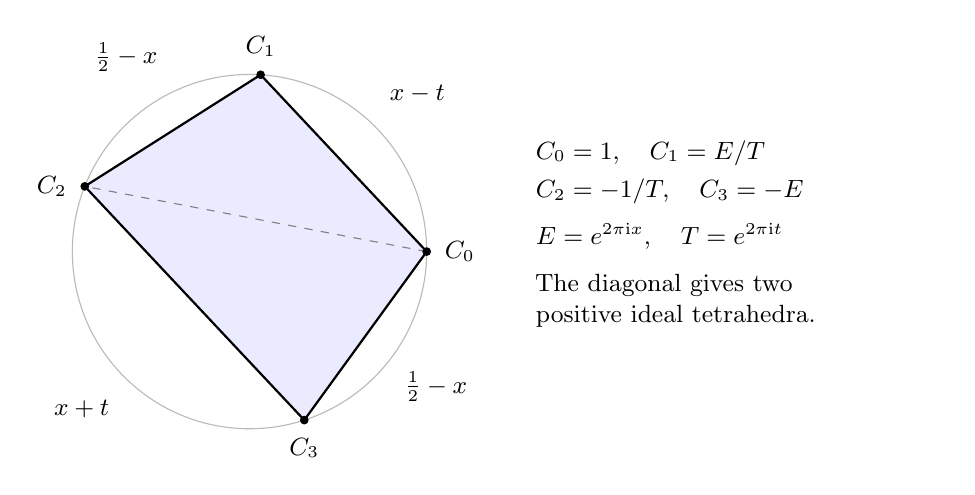
\begin{tikzpicture}[scale=2.25,every node/.style={font=\small}]
\coordinate(c0) at (1,0);
\coordinate(c1) at ({cos(86.4)},{sin(86.4)});
\coordinate(c2) at ({cos(158.4)},{sin(158.4)});
\coordinate(c3) at ({cos(288)},{sin(288)});
\draw[gray!55] (0,0) circle(1);
\fill[blue!8] (c0)--(c1)--(c2)--(c3)--cycle;
\draw[thick] (c0)--(c1)--(c2)--(c3)--cycle;
\draw[dashed,gray] (c0)--(c2);
\foreach \p/\lab/\pos in {c0/C_0/right,c1/C_1/above,c2/C_2/left,c3/C_3/below}
 {\fill(\p) circle(.7pt);\node[\pos=3pt] at(\p){$\lab$};}
\node at ({1.3*cos(43.2)},{1.3*sin(43.2)}) {$x-t$};
\node at ({1.3*cos(122.4)},{1.3*sin(122.4)}) {$\frac12-x$};
\node at ({1.3*cos(223.2)},{1.3*sin(223.2)}) {$x+t$};
\node at ({1.3*cos(324)},{1.3*sin(324)}) {$\frac12-x$};
\node[align=left,text width=5.1cm] at (2.75,.1)
 {$C_0=1,\quad C_1=E/T$\\[3pt]
  $C_2=-1/T,\quad C_3=-E$\\[6pt]
  $E=e^{2\pi\ii x},\quad T=e^{2\pi\ii t}$\\[6pt]
  The diagonal gives two\\positive ideal tetrahedra.};
\end{tikzpicture}

\caption{The boundary-plane coordinates of the mixed pyramid for
$x=0.30$, $t=0.06$. The apex is $\infty$.
The four successive half-arcs shown here are the actual parameters
of \eqref{cf:mixed-leaf}. At $t=0$ the quadrilateral becomes the
rectangle of the complete leaf.}
\label{cf:leaf-figure}
\end{figure}

Its ordered cross ratio and normalized fourth vertex are
\begin{equation}\label{cf:R}
\begin{split}
 \kap&=\frac{\sin\pi(x-t)\sin\pi(x+t)}{\cos^2\pi x}
                       =e^{-g_x},\\
 R&=\frac1{1+\kap}
    =\frac{\cos^2\pi x}{\cos^2\pi t}
    =\frac{T(1+E)^2}{E(1+T)^2}.
\end{split}
\end{equation}
Normalize its ordered base to $(0,\infty,1,R)$.
The plus-$t$ apex is
\begin{equation}\label{cf:flags}
 Z=\frac{1+E}{1+T},\qquad
 Z^2-(1+E)Z+ER=0.
\end{equation}
The other root is $TZ$, the apex of the minus-$t$ leaf in this
same normalization. The second projection chart is the reflected
minus-$t$ chart, whose apex is $Z/E$. It is not the reflection
of the plus-$t$ apex when $t\ne0$.

These formulas now define holomorphic projective coordinates
for complex $x,t$ near the complete point.
Reflection of coefficients is implemented by replacing the
phase variables by their reciprocals. Thus the reflected
minus apex is algebraically $Z/E$, without antiholomorphic
dependence on a parameter. Every defining face-map triple remains
pairwise distinct after shrinking the neighborhood; the two
auxiliary fixed points themselves coalesce at completeness.

\subsection{Whole complex face matching}
In the normalized chart the four white or completion maps are
\begin{equation}\label{cf:white}
\begin{aligned}
 W_0&=\begin{pmatrix}1&0\\0&E\end{pmatrix},&
 W_1&=\begin{pmatrix}1&E-1\\0&E\end{pmatrix},\\
 W_2&=\begin{pmatrix}E-R&R(1-E)\\E-1&1-ER\end{pmatrix},&
 W_3&=\begin{pmatrix}R&0\\1-E&ER\end{pmatrix}.
\end{aligned}
\end{equation}
The pure shaded map and the two odd cross-copy maps are
\begin{equation}\label{cf:shaded}
 S=\begin{pmatrix}0&-ER\\1&-1-E\end{pmatrix},\quad
 A=\begin{pmatrix}R&-R\\1&ER-1-E\end{pmatrix},\quad
 B=\begin{pmatrix}R/E-1-1/E&R\\-1&R\end{pmatrix}.
\end{equation}
All matrices are projective. For a mixed leaf, $W_0,W_2$
fix their two main corners and send $Z$ to $Z/E$.
The apex equation \eqref{cf:flags} verifies this last statement
also for $W_2$. The shaded assignments are
\[
 S:(Z,\infty,1)\mapsto(Z,0,R),\quad
 A:(Z,\infty,1)\mapsto(Z/E,R,0),\quad
 B:(Z,R,0)\mapsto(Z/E,\infty,1).
\]
Each is the map of the original labeled triangle.
The expressions $W_1,W_3$ are not extra leaf faces:
their actual white pieces come from its adjacent prism.

To check those pieces throughout the expression, keep the
original prism formula with complex wire parameters.
Write
\[
 \alpha=e^{2\pi\ii(z-x)},\quad
 \beta=e^{2\pi\ii(x+y-z)},\quad
 \gamma=e^{2\pi\ii(z-y)}.
\]
Its world coordinates are
\begin{equation}\label{cf:prism}
\begin{split}
 v_0&=1,\quad v_1=\alpha,\quad
 v_2=\alpha\beta,\quad v_3=\alpha\beta\gamma,\\
 P&=1+\alpha-
 \frac{\alpha[\alpha\beta(1+\gamma)-1-\alpha]}
                    {\alpha^2\beta^2\gamma-\alpha}.
\end{split}
\end{equation}
The lower, upper and output ordered quadrilaterals are
$(v_0,v_1,P,\infty)$, $(\infty,P,v_2,v_3)$ and
$(v_0,v_1,v_2,v_3)$, with wire phases
$\beta\gamma,\alpha\beta,\alpha\beta\gamma$.
For an ordered tuple $(a,b,c,d)$ let
\[
 M_{a,b,c}(z)=\frac{(z-a)(c-b)}{(z-b)(c-a)},\qquad
 R=M_{a,b,c}(d).
\]
Its world white maps are $M^{\#\, -1}W_jM$, where $\#$ reciprocates
$\alpha,\beta,\gamma$. At a real strict prism this agrees with
reflection; it is a holomorphic rational prescription in general.

The exact rational identities
\begin{equation}\label{cf:nine}
\begin{aligned}
 W_{F,1}=W_{G,1}=W_{o,1}&=W_{\rm top},&
 W_{F,3}=W_{G,3}=W_{o,3}&=W_{\rm bottom},\\
 W_{F,2}&=W_{G,0},&
 W_{o,0}=W_{F,0},\qquad W_{o,2}&=W_{G,2}
\end{aligned}
\end{equation}
are \cite[equation~(5.5)]{Geometry}. Their proof is a
rational substitution in three independent phase variables, so
it already proves \eqref{cf:nine} off the real chamber.
Here the top and bottom maps carry the original white triangles
$(P,v_1,v_2)$ and $(\infty,v_0,v_3)$ to their reflected charts.
No equality merely of absolute cross ratios is being used.

At an internal wire, \eqref{cf:local-differential} says that
the child output derivative is $g_x$ or the corresponding
stationary product derivative. The internal critical equations
therefore match the full complex cross ratios under the
same original vertex assignments as at completeness.
Three matched vertices fix a Möbius map, and the cross-ratio
equation matches the fourth. The former quadrilateral need not
remain planar; the argument matches its four flags and both
triangles of any fixed subdivision.

Turns and closure use
$T_Q(z)=(R-1)/(z-1)$ and $C_Q(z)=(z-R)/(z-1)$, with identities
\begin{equation}\label{cf:turn}
\begin{split}
 T_QW_{j+1}(E,R)&=W_j(E^{-1},1-R)T_Q,\\
 C_QW_j(E^{-1},R)&=W_{2-j}(E,R)C_Q .
\end{split}
\end{equation}
These are \cite[equation~(5.6)]{Geometry}, again rational
identities. Induction through \eqref{cf:nine} and
\eqref{cf:turn} proves that every triangular piece of a given
original white face has the same entire map. In particular the
parent prism supplies $W_1,W_3$ at every elementary cap edge.
The two completed root children ensure that the closing seams
are white. This is the specific place where the grammar
\eqref{cf:grammar} is retained.

\subsection{Relations and positivity on the retained chain}
Let $S^\#=S(E^{-1},R)$. Direct multiplication gives
\begin{equation}\label{cf:edge-words}
\begin{gathered}
 W_0S=S^\#W_0,\qquad W_2S=S^\#W_2,\qquad W_3S=S^\#W_1,\\
 W_0^{-1}BW_2^{-1}A=I,\quad
 W_2^{-1}BW_0^{-1}A=I,\quad
 W_1^{-1}BW_3^{-1}A=I.
\end{gathered}
\end{equation}
The first row is the pure edge return; the second is the odd
return, including its translational part. These are identities
for independent $E,R$, as proved in
\cite[equations~(5.7)--(5.8)]{Geometry}.
The original cut balls have a dual two-skeleton with generators
the paired faces and relations precisely these edge cycles and
the white seams. Since \eqref{cf:nine} identifies the whole
white maps, all those relations hold. The family is consequently
a representation of the original $\pi_1(Y^\eps_E)$.
The deformed image of a half ball is not assumed to be an
embedded convex polyhedron.

For later use, retain a compatible triangulation of the complete
cells. First perform the actual assembly to the single complete
polyhedron $P_E$. Its finitely many ideal vertices are distinct
by the incidence proof in \cite[Section~3]{Geometry}.
Choose an order on these vertices, and restrict it to every
constituent cell and its faces. The pulling triangulations agree
on internal quadrilaterals, since these are now the same labeled
face in $P_E$, regardless of the earlier turn or attachment order.
Coning from the first vertex to faces not containing it gives
nondegenerate tetrahedra. The vertex order chooses their diagonals;
each tetrahedron is oriented by the ambient oriented cell, rather
than by the increasing global vertex order. In that orientation
each complete shape is positive.
Use the identical subdivision in the second labeled copy.
All nontriangular external face pairings are the white maps
between corresponding copies, so their subdivisions match.
The pure and odd shaded pairings may permute vertices, but their
faces are already triangles and contain no diagonal to choose.
Thus no order on quotient cusp vertices, which could identify
many different cut vertices, is assumed.
Transport these finitely many vertices by the formulas above.
Their complete tetrahedra are positive, so their shapes remain
in the positive half-plane in one common small parameter
neighborhood. The full face maps match their triangles and
edge relations. We have the same oriented ideal fundamental
chain and the same peripheral marking as at completeness.
This construction does not require an ideal triangulation of
the subsequently filled manifold.

\section{Primitive logarithms and the unfilled cusps}
\label{cf:peripheral}

For a peripheral element fixing a selected flag, its similarity
multiplier means the coefficient of its affine action after
that flag is sent to $\infty$. At a finite flag $Z$ it is the
reciprocal of the derivative at $Z$. These are projective
similarity multipliers, twice the usual selected eigenvalue
logarithms. All logarithms below are their small branches,
zero at completeness.

The original disk and meridian words are the ones already
traced at completeness:
\begin{equation}\label{cf:peripheral-words}
 \lambda=W_2^{-1}W_0,\qquad
 \mu_0=S^{-1},\qquad
 \mu_-=A^{-1}W_0,\qquad
 \mu_+=W_0^{-1}B.
\end{equation}
They remain the same based curves in the original cut.
Their primitiveness and orientations are
\cite[equations~(7.1)--(7.5)]{Geometry}; in particular it is
the actual disk longitude, not a multiple read from an eigenvalue.
Their selected common flag is $Z$.
Put
\begin{equation}\label{cf:rhoQ}
 \rho=\frac{Z}{1+E-Z}=\frac1T,\qquad
 Q=\frac{E-Z}{Z-1}=\frac{ET-1}{E-T}.
\end{equation}
Inverting derivatives at $Z$ in
\eqref{cf:peripheral-words} gives the exact multipliers
\begin{equation}\label{cf:multipliers}
 \lambda:Q^2,\qquad
 \mu_0:\rho,\qquad
 \mu_-:\rho Q,\qquad
 \mu_+:\rho/Q.
\end{equation}
For example the fixed-point equation of $S$ is precisely
\eqref{cf:flags}, and substitution in the Möbius derivative
$\det S/(cZ+d)^2$ gives the first meridian factor.
The same substitution gives the other three factors.
At $t=0$ both $\rho$ and $Q$ equal one, so no central logarithmic
constant can enter their small branches.

From \eqref{cf:g} and \eqref{cf:rhoQ} one has
$Q=e^{-v}$ and $\rho=e^{-2\pi\ii t}$.
It follows that the original signed meridian and disk longitude
have logarithms
\begin{equation}\label{cf:primitive-logs}
 U=-2\pi\ii t+\eps v=-2\pi\ii\chi,\qquad V=-2v.
\end{equation}
Using the envelope rule proves \eqref{cf:UV}.
The half-twist part of $G=2\pi\ii\Phi_\eps$ is
$-\eps V^2/8$ at each leaf, exactly the shear in
\eqref{cf:local-potential}.

All main cusps also retain their actual peripheral words.
At corner $C_j$ the small main meridian is
$W_{j-1}^{-1}W_j$, or its inverse according to orientation.
Both factors fix that corner. Their derivatives are equal:
$E^{-1}$ at $C_0,C_2$ and $E$ at $C_1,C_3$, using the
finite coordinate at infinity. Thus the meridian multiplier
is identically one. It is nonidentity at the complete point,
and remains so nearby; hence it is parabolic.
Every element commuting with a nonidentity parabolic Möbius
map is a translation in its fixed-flag chart.
The original main longitude commutes with this meridian.
Its multiplier is therefore also one. This verifies
the entire unfilled main peripheral group, not just a
trace equation at a single corner.

The selected auxiliary flags, the main flags and all face
maps vary holomorphically and stay in bounded frames near
their complete values. A finite collection of charts suffices.
We may therefore choose one neighborhood where the actual
framed family and all the positive tetrahedra constructed above
are simultaneously defined.

\section{The primitive solution for independently signed slopes}
\label{cf:critical}

Put $r_\ell=1/p_\ell$ and solve
\begin{equation}\label{cf:r-equations}
 V_\ell(\boldsymbol\chi)+r_\ell U_\ell(\boldsymbol\chi)
                       =-2\pi\ii r_\ell .
\end{equation}
At $\mathbf r=0$ the solution is $\boldsymbol\chi=0$.
Lemma~\ref{cf:hessian} and \eqref{cf:UV} give
\begin{equation}\label{cf:Jacobian}
 D_{\boldsymbol\chi}V(0)=-2\pi\ii\,\diag(\tau_1,\ldots,\tau_H).
\end{equation}
It is invertible because $\Ima\tau_\ell>0$.
The holomorphic implicit-function theorem gives a unique solution
$\boldsymbol\chi_*(\mathbf r)$ on one fixed polydisk in all the
independent reciprocal slopes. Shrink that polydisk so that its
image lies in the framed neighborhood of
Section~\ref{cf:peripheral}. For real signed integer $p_\ell$
this requires only a lower bound on each $|p_\ell|$.
There is no constraint on their ratios.

When $p_\ell\ne0$, \eqref{cf:r-equations} is exactly
\begin{equation}\label{cf:slope-equations}
 U_\ell+p_\ell V_\ell=-2\pi\ii .
\end{equation}
By \eqref{cf:UV} these are precisely the critical equations of
\eqref{cf:action}. Thus local uniqueness applies to the stated
critical point, not only to a separate system of period equations.

There is also a direct classical check that the filled auxiliary
groups have a genuine loxodromic direction. Separate evenness of
$\Phi_\eps$ gives holomorphic functions $\widetilde\tau_\ell$
such that
\[
 V_\ell=\widetilde\tau_\ell(\boldsymbol\chi)\,U_\ell,\qquad
 \widetilde\tau_\ell(0)=\tau_\ell .
\]
In fact divide $\partial_{\chi_\ell}\Phi_\eps$ by $\pi\ii\chi_\ell$;
the apparent singularity is removable. Shrink the neighborhood
so $\Ima\widetilde\tau_\ell>0$ throughout it.
At the solution of \eqref{cf:r-equations},
\begin{equation}\label{cf:sign}
\begin{split}
 \chi_{\ell,*}
  &=\frac{r_\ell}
          {\widetilde\tau_\ell(\boldsymbol\chi_*)+r_\ell},\\
 \Rea V_\ell
  &=\frac{2\pi r_\ell^2\,
          \Ima\widetilde\tau_\ell(\boldsymbol\chi_*)}
           {|\widetilde\tau_\ell(\boldsymbol\chi_*)+r_\ell|^2}
       >0 .
\end{split}
\end{equation}
The second formula holds for either sign of the nonzero real
$r_\ell$. Thus the longitude multiplier has nonunit modulus.
The sign is derived from the classical potential and the original
positive cusp ratio, without a source noncancellation argument.

\section{From a peripheral equation to the original smooth filling}
\label{cf:metric}

We now apply a metric result, rather than identifying an
exponential equation with a filled metric.
The following is the precise input
\cite[Proposition~6.1]{Marked}.

\begin{proposition}[Near-complete primitive completion, imported]
\label{cf:completion-input}
Let $M$ be an oriented complete finite-volume hyperbolic
three-manifold with torus cusps and complete holonomy $\rho_0$.
Fix primitive bases $(\mu_i,\lambda_i)$.
There is one neighborhood of $\rho_0$ with its peripheral fixed
flags, chosen before any slopes, with the following property.
Let $\rho$ be an actual representation in that neighborhood and
$U_i,V_i$ its small similarity logarithms in bounded frames
sending the flags to infinity. Suppose both multipliers are one
at each cusp to remain unfilled. At each cusp to be filled suppose
$a_iU_i+b_iV_i=\pm2\pi\ii$ with $\gcd(a_i,b_i)=1$.
Then $\rho$ descends to the original topological filling and
is its smooth complete finite-volume hyperbolic holonomy.
\end{proposition}

This statement supplies completion; it does not supply the
representation or solve its equations. Its hypotheses hold here
for the following concrete reasons.
The complete manifold is the actual $Y^\eps_E$ of
\cite[Theorem~1.2]{Geometry}. Its primitive bases are the traced
curves \eqref{cf:peripheral-words}. The rational face maps and
original cut relations prove an actual framed representation
near that holonomy, in bounded charts. Section~\ref{cf:peripheral}
proves that every main peripheral group is a translation group.
The equations at the auxiliary cusps are
\eqref{cf:slope-equations}; their slopes are primitive because
$(1,p_\ell)$ is a primitive integer vector in the original basis.
These facts verify every premise of
Proposition~\ref{cf:completion-input}.

For clarity, we spell out the winding step in that proposition
and its relation to the present markings. On a compact truncated
core, a finite partition of unity in the future hyperboloid
model averages the small change of complete developing maps:
\begin{equation}\label{cf:core}
 \begin{split}
 Y_\rho(x)&=\sum_{j,\gamma}
       \eta_{j,\gamma}(x)\rho(\gamma)\rho_0(\gamma)^{-1}x,\\
 E_\rho(x)&=\frac{Y_\rho(x)}
       {\sqrt{-\langle Y_\rho(x),Y_\rho(x)\rangle}} .
 \end{split}
\end{equation}
Here the $\eta_{j,\gamma}$ are equivariant lifts of a finite
partition on evenly covered balls. A positive sum of future
timelike vectors is timelike. Reindexing proves equivariance,
and on a compact fundamental part $E_\rho$ is $C^1$-close to
the complete identity map. It is therefore a positive local
diffeomorphism. This argument assumes no discreteness of
the deformed representation.

For one complete cusp use coordinates
$(w,s)\in\CC\times[s_0,\infty)$ with translation lattice
$\Lambda$. In the moving flag frame its peripheral maps are
$A_\lambda(z)=a_\lambda z+b_\lambda$.
Choose a smooth compactly supported partition satisfying
$\sum_{\lambda\in\Lambda}\eta(w-\lambda)=1$, and put
\begin{equation}\label{cf:link}
\begin{split}
 d_\rho(w)&=\sum_{\lambda\in\Lambda}
            \eta(w-\lambda)A_\lambda(w-\lambda),\\
 F_\rho(w,s)&=\bigl(d_\rho(w),e^{s+\xi_\rho(w)}\bigr),
\end{split}
\end{equation}
where $\xi_\rho$ is the real-linear extension of
$\lambda\mapsto\log|a_\lambda|$.
Then $d_\rho(w+\lambda)=A_\lambda d_\rho(w)$.
Its real Jacobian is positive on a compact fundamental
parallelogram, by closeness to the identity, and equivariance
propagates this everywhere. The Jacobian of $F_\rho$ is
$e^{s+\xi_\rho(w)}\det_{\RR}Dd_\rho(w)>0$.
Interpolation with \eqref{cf:core} on a compact collar remains
$C^1$-close and positive.
This constructs an actual nonsingular hyperbolic metric on
the original core and its ideal-end-deleted cusps.

At a cusp to be filled, \eqref{cf:sign} in particular gives
a multiplier different from one. Commuting affine maps have
a common finite fixed point $q$, in addition to infinity.
For any generator with $a\ne1$ it is $q=b/(1-a)$.
Both complete generator translations are nonzero, while their
multipliers tend to one. Thus $|q|\to\infty$ uniformly near
completeness, even if one generator has multiplier one.
The developed fundamental parallelogram and its fixed generator
paths remain in a bounded set and have bounded lengths.
They therefore miss $q$ in one sufficiently small neighborhood.
Equivariance extends this exclusion to the entire link cover.

On that simply connected cover choose
$f=\Log(d_\rho-q)$. The metric $|df|^2$ is nonsingular and
descends to a compact torus; it is complete. Its lifted
Euclidean developing map covers $\CC$, by lifting finite line
segments. Since the plane is simply connected, $f$ is a
global diffeomorphism and its periods form a rank-two lattice.
For a fixed generator path of developed length at most $L$,
inside $|d_\rho|\le R$,
\begin{equation}\label{cf:small-period}
 |\Delta f|\le \frac{L}{|q|-R}\longrightarrow0.
\end{equation}
Its exponential is the actual affine multiplier. Consequently
the increment equals its prescribed small logarithm, with
no extra $2\pi\ii$ integer. Thus the two actual periods are
$U,V$ before the potentially large coefficient $p$ is used.
This is why the fixed neighborhood controls all independently
long slopes.

Translate $q$ to zero. Periodicity bounds
$e^{s_0+\xi_\rho(w)}/|d_\rho(w)-q|$, so the end contains
a full epigraph $y>A|d_\rho-q|$.
Set
\[
 r=\frac{y}{|d_\rho-q|},\qquad
 R=\operatorname{arsinh}(1/r),\qquad
 \theta=\Ima f,\qquad
 X=\Rea f+\tfrac12\log(1+r^2).
 \]
Direct substitution gives
\begin{equation}\label{cf:tube}
 ds^2=dR^2+\cosh^2R\,dX^2+\sinh^2R\,d\theta^2 .
\end{equation}
The epigraph contains a whole punctured tube $0<R<R_0$.
A period $L$ translates $(X,\theta)$ by $(\Rea L,\Ima L)$.
The original slope $\mu+p\lambda$ has period $-2\pi\ii$,
exactly one angular turn. Its complementary primitive period
$V$ has nonzero real part, either by rank two of the period
lattice or directly by \eqref{cf:sign}.
Adding the axis gives a smooth solid torus, with precisely
the original slope as meridian. Its holonomy is the identity:
it fixes both $q,\infty$ and has multiplier one.
This proves group descent, rather than merely an exponential
relation. Reversing the angular sign reverses its parametrization,
not the metric orientation.

\begin{figure}[ht]
\centering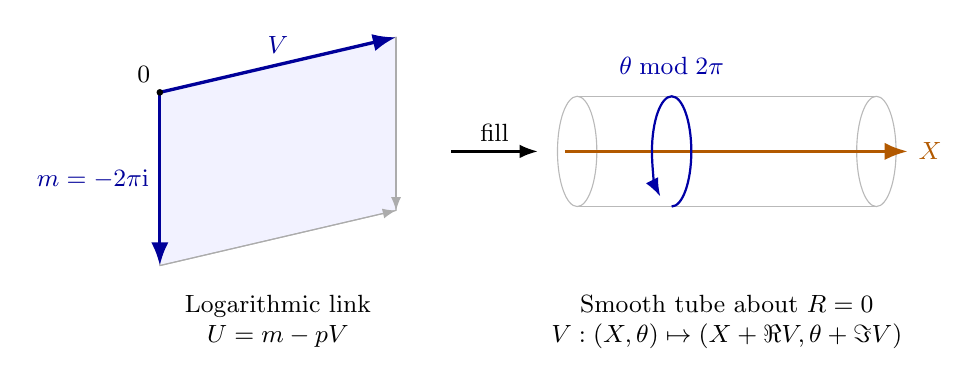
\begin{tikzpicture}[x=1cm,y=1cm,>=Latex,font=\small,
 period/.style={very thick,->,blue!60!black},
 boundary/.style={thin,gray!65}]
 \begin{scope}[shift={(0,0)}]
  \coordinate (o) at (0,1.8);
  \coordinate (m) at (0,-.4);
  \coordinate (v) at (3,2.5);
  \coordinate (mv) at (3,.3);
  \fill[blue!5] (o)--(v)--(mv)--(m)--cycle;
  \draw[boundary] (o)--(v)--(mv)--(m)--cycle;
  \draw[period] (o)--(m) node[midway,left] {$m=-2\pi\ii$};
  \draw[period] (o)--(v) node[midway,above] {$V$};
  \draw[->,gray!65] (m)--(mv);
  \draw[->,gray!65] (v)--(mv);
  \fill (o) circle (1.2pt);
  \node[above left] at (o) {$0$};
  \node[below,align=center] at (1.5,-.65)
       {Logarithmic link\\$U=m-pV$};
 \end{scope}
 \draw[->,thick] (3.7,1.05)--(4.8,1.05)
      node[midway,above] {fill};
 \begin{scope}[shift={(5.3,1.05)}]
  \draw[gray!55] (0,-.7)--(3.8,-.7);
  \draw[gray!55] (0,.7)--(3.8,.7);
  \draw[gray!55] (0,0) ellipse (.25 and .7);
  \draw[gray!55] (3.8,0) ellipse (.25 and .7);
  \draw[very thick,orange!70!black,->] (-.15,0)--(4.2,0)
      node[right] {$X$};
  \draw[blue!65!black,thick,->]
       (1.2,-.7) arc[start angle=-90,end angle=235,
                     x radius=.25,y radius=.7];
  \node[above,blue!65!black] at (1.2,.85) {$\theta\bmod 2\pi$};
  \node[below,align=center] at (1.9,-1.7)
      {Smooth tube about $R=0$\\
       $V:(X,\theta)\mapsto(X+\Re V,\theta+\Im V)$};
 \end{scope}
\end{tikzpicture}

\caption{The actual logarithmic link and its smooth filling.
The period $m=U+pV=-2\pi\ii$ is the primitive meridian of the
added solid torus; $V$ is the original disk-longitude period.
The old basis is $U=m-pV$. Equation \eqref{cf:tube} turns
$V$ into an axial translation and rotation, and $m$ into
one full angular turn.}
\label{cf:filling-figure}
\end{figure}

At an unfilled main cusp the multipliers are one. The same
compact Euclidean-link argument now gives a complete translation
plane and a full horoball quotient in \eqref{cf:link}.
The middle region is compact; the added tubes and the remaining
horoball ends have finite volume. The metric is complete.
Its universal developing map covers simply connected hyperbolic
space and hence is an isometry. The filled topology and all
its markings are the ones described in \eqref{cf:slope}.
This completes the metric part of Theorem~\ref{cf:main}.

\section{The absolute action and the filled fundamental chain}
\label{cf:volume-proof}

\subsection{The correct polarization}
Define $G=2\pi\ii\Phi_\eps$. The exact period formula
\eqref{cf:UV} gives
\begin{equation}\label{cf:primitive}
 \dd G=\frac12\sum_\ell V_\ell\,\dd U_\ell,\qquad
 \Ima G(0)=2\pi F_0=\Vol(Y^\eps_E).
\end{equation}
This is the $V\,dU$ polarization. A potential with differential
$-\frac12\sum U\,dV$ differs by the boundary term
$\frac12\sum UV$. Its regulator correction cannot be copied
unchanged into \eqref{cf:primitive}.

Let $\mathcal V(\rho_{\boldsymbol\chi})$ be the signed
ideal-tetrahedron volume of the retained original fundamental
chain from Section~\ref{cf:deformation}.
The local peripheral differential
\cite[equation~(7.3)]{Marked} is
\begin{equation}\label{cf:volume-differential}
 \dd\mathcal V
 =\frac12\sum_\ell
    \bigl(\Rea V_\ell\,\dd\Ima U_\ell
                 -\Rea U_\ell\,\dd\Ima V_\ell\bigr).
\end{equation}
Its hypotheses are present here: the oriented ideal chain is
positive and nondegenerate near the complete point; actual
face maps cancel the internal boundaries; edge relations
keep their logarithmic sums fixed; and the primitive
peripheral basis has the orientation
$\Ima(\lambda/\mu)>0$ at completeness.
All main logs vanish because their peripheral actions are
translations, so they contribute zero.
The factor $1/2$ in \eqref{cf:volume-differential} is for
similarity logarithms; replacing them by eigenvalue logarithms
without adjusting the factor would change the formula.

For reference, that local identity follows by differentiating
the Bloch--Wigner volume on each oriented tetrahedron and
cancelling paired normal-face flows. The remaining cusp
coefficient rows have intersection pairing $-2$ on the
primitive meridian/longitude basis; the inverse tangent
pairing is $-1/2$. In \cite[Section~7.1]{Marked} the signs
are computed with the positively ordered model
$(0,\infty,1,z)$ in standard upper-half-space orientation.
The original complete cusp orientation
\eqref{cf:cusp} is precisely that convention.
No complete character-variety uniqueness is an input to
this local calculation.

Taking the imaginary part of \eqref{cf:primitive} shows that
the differential of
$\Ima G-\frac12\sum\Rea U_\ell\Ima V_\ell$
is exactly \eqref{cf:volume-differential}.
At completeness its value is the actual metric volume,
by \eqref{cf:primitive}; hence the constant on this connected
neighborhood is fixed:
\begin{equation}\label{cf:regulator}
 \mathcal V(\rho_{\boldsymbol\chi})
   =2\pi\Rea\Phi_\eps(\boldsymbol\chi)
          -\frac12\sum_\ell\Rea U_\ell\,\Ima V_\ell .
\end{equation}
This is an absolute equality on the original marked chain.

\subsection{The critical boundary term}
At a real integer filling tuple, write $\chi_\ell=u_\ell+\ii v_\ell$.
The critical equation gives
$V_\ell=2\pi\ii(\chi_\ell-1)/p_\ell$.
Direct substitution yields
\begin{equation}\label{cf:boundary-cancellation}
\begin{split}
 -\tfrac12\Rea U_\ell\,\Ima V_\ell
  &=-\frac{2\pi^2}{p_\ell}v_\ell(u_\ell-1)\\
  &=2\pi\Rea\left(\frac{\pi\ii}{2p_\ell}
                              (\chi_\ell-1)^2\right).
\end{split}
\end{equation}
Thus \eqref{cf:regulator} equals
$2\pi\Rea S_{\eps,\mathbf p}(\boldsymbol\chi_*)$.
It remains to identify the same ideal-chain volume with
the complete filled metric, rather than infer that conclusion
from a differential identity.

\subsection{Keeping the same boundary triangulation}
The comparison in \cite[Section~7.3]{Marked} applies to the
primitive completion proved above. We describe its chain
content to fix the absolute interpretation.
At a filled cusp conjugate the two fixed points to $0,\infty$.
On each triangle of the retained boundary triangulation
the conical ideal development has form
$(a(w),Yb(w))$, with $b>0$.
The functions and their derivatives are bounded on a finite
fundamental set. An equivariant axis map is
$(0,Y e^{\eta(w)})$, where $\eta$ has the real peripheral
logarithmic character. On that same triangulation use
\begin{equation}\label{cf:homotopy}
 H_s(w,Y)=\left(sa(w),
     Y\exp\bigl((1-s)\eta(w)+s\log b(w)\bigr)\right),
       \qquad 0\le s\le1.
\end{equation}
It is face-compatible and equivariant: horizontal coordinates
transform by the complex multiplier and both heights by its
modulus. The height is comparable to $Y$, horizontal
derivatives are bounded, and height derivatives are $O(Y)$.
The hyperbolic volume form
$y^{-3}\,dx_1\wedge dx_2\wedge dy$ bounds this boundary
homotopy's volume by $O(Y^{-2})$.

After the primitive slope has been killed, extend the same
axis-valued triangulated boundary through the solid torus.
The remaining cyclic peripheral group acts along the axis.
All added vertices lie on that axis, so every added
tetrahedron has zero signed volume.
Unfilled main cusp comparisons have the same vanishing
boundary estimate.
Stokes on finite truncations, followed by $Y\to\infty$,
therefore identifies the original chain with the filled
equivariant fundamental class.

Compare it with the developing map of the complete metric
from Section~\ref{cf:metric}. They represent this same class
and have the same remaining cusp flags. A common subdivision,
straightening and the same vanishing boundary estimate give
\[
 \mathcal V(\rho_{\boldsymbol\chi_*})
       =\Vol\bigl(Y^\eps_E(\mathbf p)\bigr).
 \]
Using an unrelated new triangulation with axis vertices
would not prove this equality; it is the retained boundary
homotopy \eqref{cf:homotopy} that supplies the comparison.
The usual metric volume is unambiguous also by the
volume-independence statement \cite[Lemma~7.1]{Marked}.
Together with \eqref{cf:boundary-cancellation} this proves
\eqref{cf:volume} and Theorem~\ref{cf:main}.

\section{The analytic interface and finite checks}
\label{cf:interface}

The classical potential has been defined from the cell functions
\eqref{cf:m}, \eqref{cf:g} and the exact meridian shear.
An application to a finite source must separately prove that
its selected limiting leaf action is this $f_\eps$, including
the parameter-dependent constant. Matching only its $x$
derivative or its complete Hessian is insufficient.
For example the exact classical exponential relation
$R^{-1}-1=e^{-\partial_x f_\eps}$ fixes a face shape,
but does not by itself identify a finite coefficient's
normalization. One must also compare the endpoint-normalized
leaf primitive and then eliminate the same internal wires.
Control of complementary terms and a nonzero whole filling
asymptotic are further analytic assertions. None is a
premise or conclusion of Theorem~\ref{cf:main}.

The construction-specific imported inputs are the complete
stationary point of \cite[Proposition~5.3]{Newton} and the
complete metric, actual cut and primitive bases of
\cite[Theorem~1.2 and Sections~4--7]{Geometry}.
The full complex continuation uses the latter paper's
rational face identities, not a claim that a nonplanar
deformed half ball is convex. The metric completion and
peripheral-volume facts imported from \cite{Marked} have
their actual hypotheses verified above. Standard holomorphic
implicit-function theory is used only at the two explicitly
invertible Jacobians. The usual Dehn-filling and
peripheral-volume framework provides historical context
\cite{NeumannZagier}; the original words and the absolute
normalization are retained in the calculation here.

The deterministic accompanying program \texttt{check.py}
verifies exact rational flag and multiplier identities,
the local Hessian coefficient, the real signed formula
\eqref{cf:sign}, and the boundary cancellation
\eqref{cf:boundary-cancellation}. Its negative controls
detect the missing factor two between eigenvalue and
similarity logs and an incorrect shear sign.
The record includes hashes of the actual source inputs.
These checks establish finite algebraic equalities only.
They do not prove the implicit-function theorem, the original
topological identification, metric completeness, or the
fundamental-chain comparison.

\begin{thebibliography}{9}
\bibitem{Geometry}
\emph{Pyramids, prisms, and complete geometry of Conway closures},
companion paper, Theorem~1.2 and Sections~4--7.
\href{https://sashakolpakov.github.io/murakamis_dream/papers/conway-geometry.pdf}
{Companion PDF}.

\bibitem{Newton}
\emph{Newton coefficients and positive sources for Conway tangles},
companion paper, Proposition~5.3.
\href{https://sashakolpakov.github.io/murakamis_dream/papers/newton-tangles.pdf}
{Companion PDF}.

\bibitem{Marked}
\emph{Circle patterns and primitive fillings of augmented links},
companion paper, Proposition~6.1, equation~(7.3) and Section~7.3.
\href{https://sashakolpakov.github.io/murakamis_dream/papers/marked-fillings.pdf}
{Companion PDF}.

\bibitem{NeumannZagier}
W.~D.~Neumann and D.~Zagier, Volumes of hyperbolic three-manifolds,
\emph{Topology} \textbf{24} (1985), 307--332.
\href{https://doi.org/10.1016/0040-9383(85)90004-7}
{doi:10.1016/0040-9383(85)90004-7}.
\end{thebibliography}

\end{document}
